\subsection{Casos de Prueba}

Vamos a presentar 5 instancias distintas del problema mediante gráficos, y la solución que nos devuelve la implementación, de manera de hacer una comprobación visual del funcionamiento. Más abajo vemos las soluciones posibles y lo que nos devolvió el algoritmo.
Los ejemplos abarcan casos que tienen 2 soluciones y otros sólo una, y árboles con distintos grados máximos.

\begin{center}
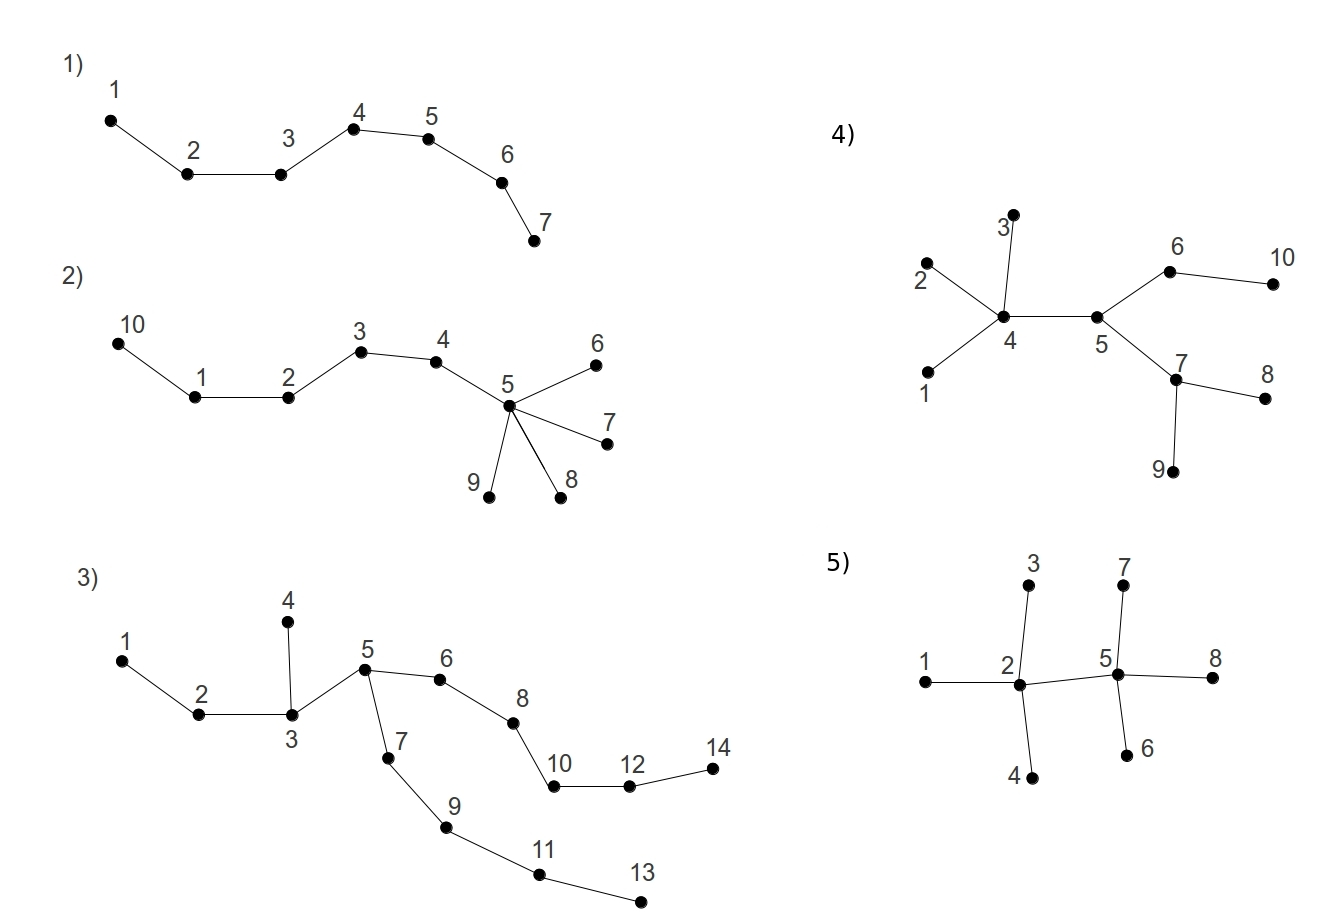
\includegraphics[scale=0.5]{ej2/2/graficos/imagen05.jpg} 
\end{center}

\begin{center}
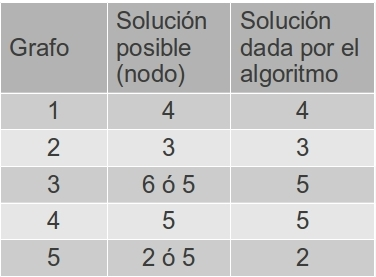
\includegraphics[scale=0.5]{ej2/2/graficos/imagen06.jpg} 
\end{center}